\begin{figure*}[tb]\centering
	\subfloat[Classification labels.]{
		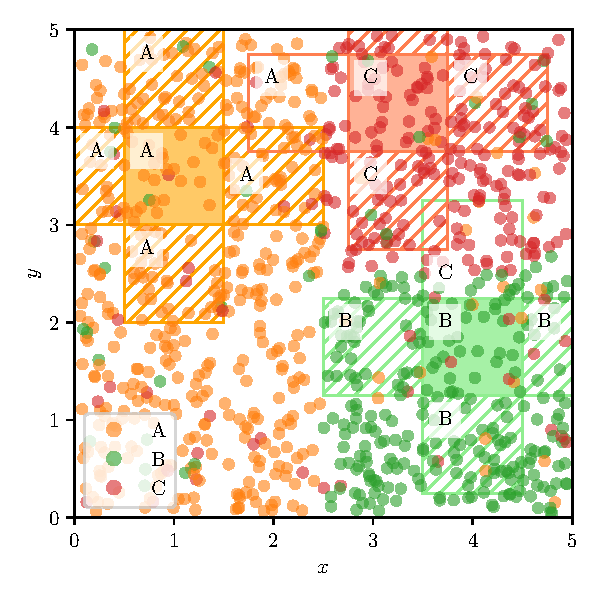
\includegraphics[width=0.295\linewidth]{figures/class-sim.pdf}\label{fig:gs1}
	}
	\subfloat[Constant outputs.]{
		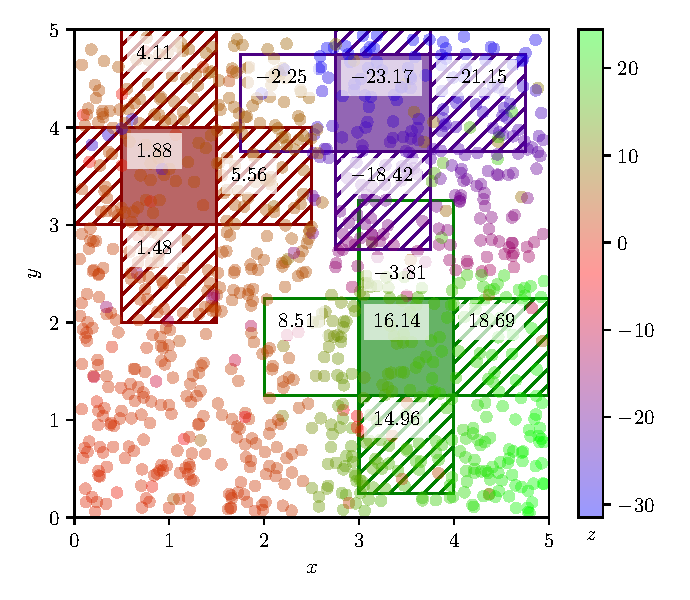
\includegraphics[width=0.34\linewidth]{figures/const-sim.pdf}\label{fig:gs2}
	}
	\subfloat[Regression laws.]{
		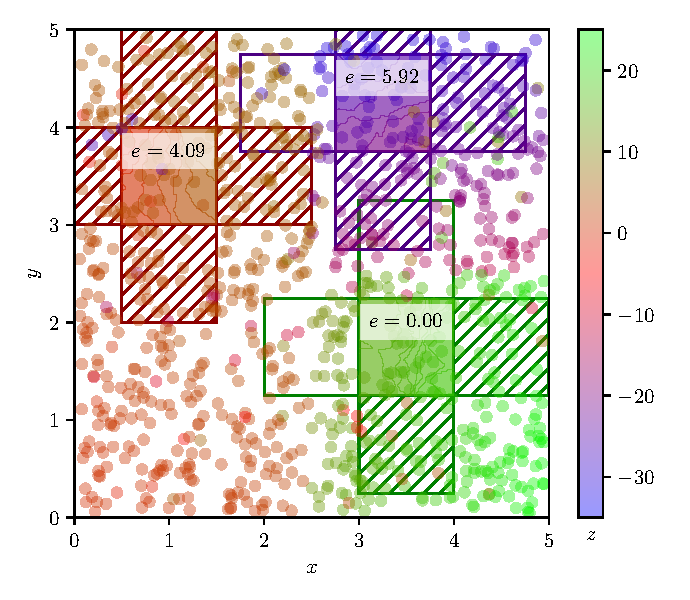
\includegraphics[width=0.34\linewidth]{figures/regr-sim.pdf}\label{fig:gs3}
	}
	\caption{Two-dimensional example of different similarities calculated for generalised extractors. Hatched regions are suitable to be merged with the adjacent one (coloured background).}\labelfig{general-sim}
\end{figure*}
